% Generated by thesis/ch7/exp1/networks.py -- do not edit by hand.
\begin{figure}[!htbp]
  \centering
  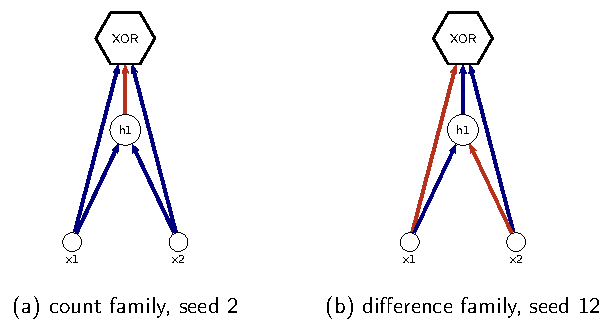
\includegraphics[width=\textwidth,height=0.8\textheight,keepaspectratio]{figures/exp1/networks/xor-raw}
  \caption{XOR: one minimal network of each family, reduced, before any explanation. (a) Count family; (b) difference family. Bottom: the input columns; circles h1, h2, \ldots: hidden units; hexagon: the output. Edges: blue, a positive weight (raises the score); red, a negative weight (lowers it); thicker, a larger weight.}
  \label{fig:exp1-net-xor-raw}
\end{figure}
